%!TEX root = ../../../main.tex

\chapter{Coupling of \Nds to Photonic Structures}	\label{ch::coupling}
\chaptermark{Photonic Structures}

	In the previous chapter, we reported on \pl properties of different sets of \sivs.
	Across the available samples, emitters were found to exhibit considerable variations in wavelength, \lw as well as intensity of \zpls.
	This broad variety in combination with the ability to examine \sivs individually opens up the possibility to preselect emitters according to desired spectroscopic parameters, such as narrow \lw{}s, high count-rates and single photon emission.

	Once suitable emitters are identified, their host \nds can be moved with precision using \pp methods.
	In particular, \sivs may be transfered and coupled to photonic structures where their extraordinary properties can be exploited to create \sps.
	Such sources are useful tools, widely required for applications in metrology and various quantum technologies such as quantum computing or quantum cryptography.

	In the scope of this thesis, \nds including suitable \sivs were identified and coupled to two different kinds of structures: \Vcsels (\VCSELs) and plasmonic nano-antennas.

	To create a hybrid-integrated \sps, a \nd containing an \siv placed on top of a \VCSEL. The \siv is positioned such that it is directly pumped by the \VCSEL output laser beam. Thus, the emission of the \siv is steered indirectly via the operation of the \VCSEL. Through the use of suitable optical filters allowing only \siv \fl to emerge, a controlled \sps can be realized. This system is interesting in the context of metrological applications, as it constitutes a promising building block for a portable device ready to calibrate single photon detectors.

	Coupling \sivs to plasmonic nano-antennas aims at enhancing the detectable \pl intensity of an emitter.
	As described in previous chapters, not only \ZPL position and \lw, but also the \pl intensity varies strongly among individual \sivs.
	As mentioned we aim to add momentum to the adaption of the quantum candela. To this end \spss are needed as calibration devices for the development of photon-counting detectors. \Spss exhibiting a high intensity are favorable for calibration purposes \cite{Vaigu2017}. Furthermore, plasmonic antennas can be used to tune the emitters' \pl spectrum.



	\section{Additional Experimental Methods} \label{sec::methods_coupling}

	Coupling \sivs to photonic structures requires specialized experimental methods.
	A range of challenges must be overcome:
	First, additionally to the spectroscopic preselection, the \pp process poses further technical restrictions on the suitability of a host \nd.
	The size of the host \nd has to be bigger than \SI{70}{nm} and they have to lie isolated on the substrate surface, i.e. with a distance of about one micrometer.
	This substantially reduces the number of \siv candidates ready to be coupled to photonic structures.
	Another challenge is posed by accurately picking up a single \nd hosting an \siv and placing it precisely at a specified position within a given photonic structure.
	Furthermore, since the \siv is to function as the \pl emitter, it must not be damaged during the relocation process.
	To minimize both the damage cause by electron radiation, both the dose and the energy are minimized.
	Hence, the \pp process is performed as fast as possible and with a low acceleration voltage that is just strong enough to see a hazy image of the \nd.


	In the context of this thesis we explored the following methods to couple \nds to photonic structures:

	\begin{enumerate}
		\item Directly spin-coat the target structures with a \nd solution and consecutively look for a structure containing a \nd with an \siv exhibiting the desired spectroscopic properties. Frankly, this method relies on chance and is only feasible for the application with antenna structures due to the large number of antennas on one substrate. It is not advised to be used with \VCSELs because of their morphology and the small number of \VCSELs on an individual piece of substrate.

		\item Identify \nds containing suitable \sivs and individually relocate them to the destination structure using the tip in a \sem to perform a \pp routine. For this method to be effective, \nds must have a certain size. The obvious advantage of this method is the fact that only the very best emitters are used. Furthermore, the \pp process can be monitored in real-time. On the other hand, the electron radiation present during the \pp process may damage the \siv, introducing a risk of completely invalidating an emitter.

		\item Identify \nds containing suitable \sivs and individually relocate them to the destination structure using an \afm to perform a \pp routine. While this method has the advantage that the \nds are not irradiated with electrons, the disadvantage is that it is not possible to  observe the picking process in real time. As a consequence, the area of the preselected \nd has to be scanned after every pick-up attempt, which is prohibitively time consuming and therefore was not further pursued after initial trials.
	\end{enumerate}

		In the following we detail the \pp technique since it the key technique in this chapter. We also discuss the properties of the nano-manipulator and how we identify \nds suitable for \pp transfer. The \pp process itself is very fickle and difficult to execute correctly. We are grateful for the guidance and support provided by \pauly in addition to the nano-manipulator setup itself.
		\\
	\subsection{Nano-manipulator} \label{subsec::nanomanipulator}

		The nano-manipulator used for our experiments (Kleindiek, model MM3A-EM) has a exchangeable tungsten tip
	  mounted inside a Thermo Scientific\texttrademark{} Helios NanoLab\texttrademark{} DualBeam\texttrademark{} microscope. This device combines a \fib and an electron microscope.
		The bent nano-manipulator tip can bee seen in \autoref{fig::nanomanipulator_image} has $3$ degrees of freedom: up/down and left/right both in an arc up to \SI{240}{\degree}, and \SI{12}{\milli\metre} in/out.

		\begin{figure}[htp]
				\centering
				\testbox{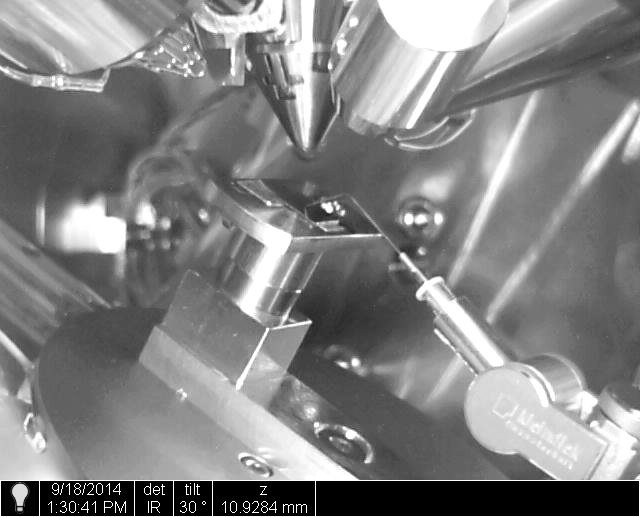
\includegraphics[trim = 0 0 0 0,  clip= true, width = 0.5\textwidth]{./pics/nanomanipulator_image_arrows.png}}
				\label{fig::nanomanipulator_image}
			\caption[Nano-manipulator in a SEM setup]{Image of the nano-manipulator mounted in the FIB. The arrows indicate the degrees of freedom of motion of the nano-manipulator. The custom made workbench is situated in the middle of the picture. On top of it, there is a \SI{1}{\centi\meter\squared} substrate with coated \nds, the nano-manipulator tip pointing to the middle of it. Behind it, there is the target \vcsel. Perpendicular to the workbench, the objective of the electron microscope can be seen. The angled cone perpendicular to the top edge of the image is the objective of the \fib.}
		\end{figure}

		Before using the nano-manipulator, its tip was ``sharpened'' with a focused ion beam by etching away tungsten with gallium ions. Its final radius of curvature amounts to \SI{100}{\nano\meter}. The sharpening enables the pick-up of \nds of a size suitable for use with photonic structures.
		In \autoref{subfig::nanomanipulator_tip} two sharpened tips are shown.

		\begin{figure}[htp]
			\begin{subfigure}[t]{ 0.49\linewidth}
				\centering
				\testbox{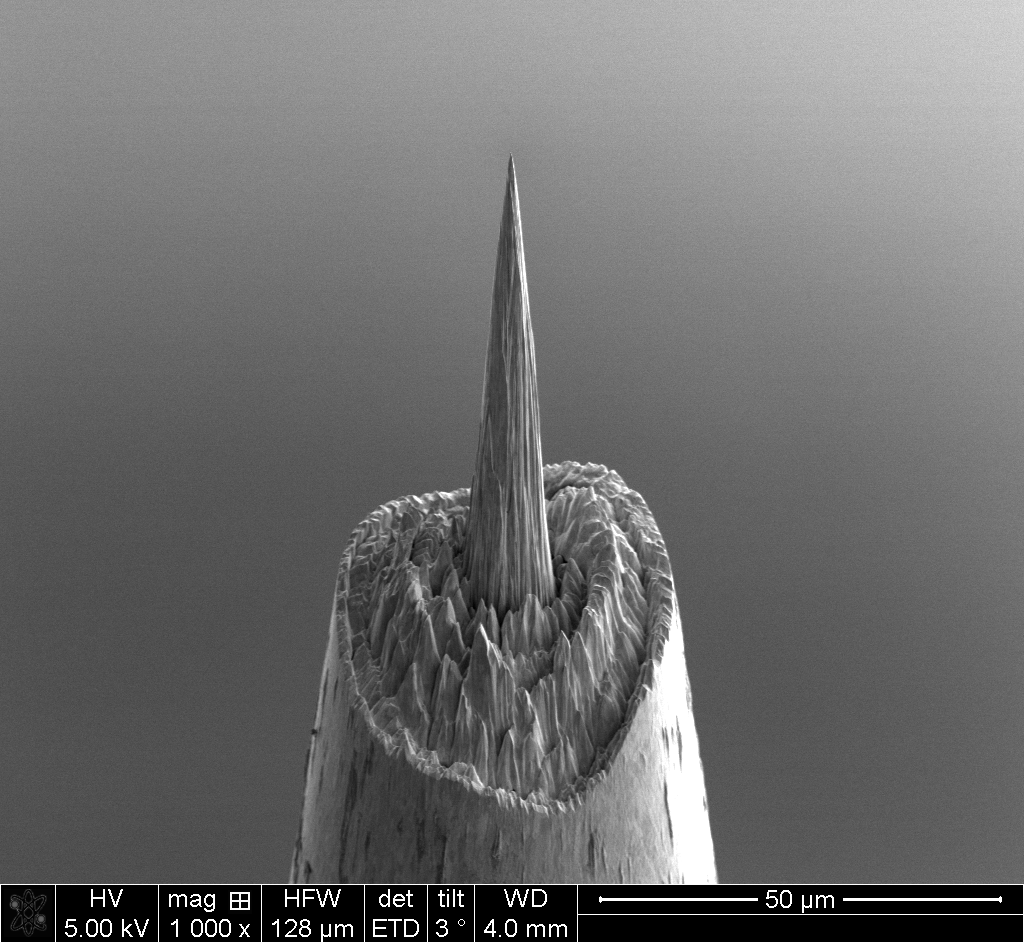
\includegraphics[trim = 0 0 0 0,  clip= true, width = \textwidth]{./pics/Tip2_140826_03.png}}
				\caption{}
				\label{subfig::nanomanipulator_tip}
			\end{subfigure}
			\hfill
			\begin{subfigure}[t]{ 0.49\linewidth}
				\centering
				\testbox{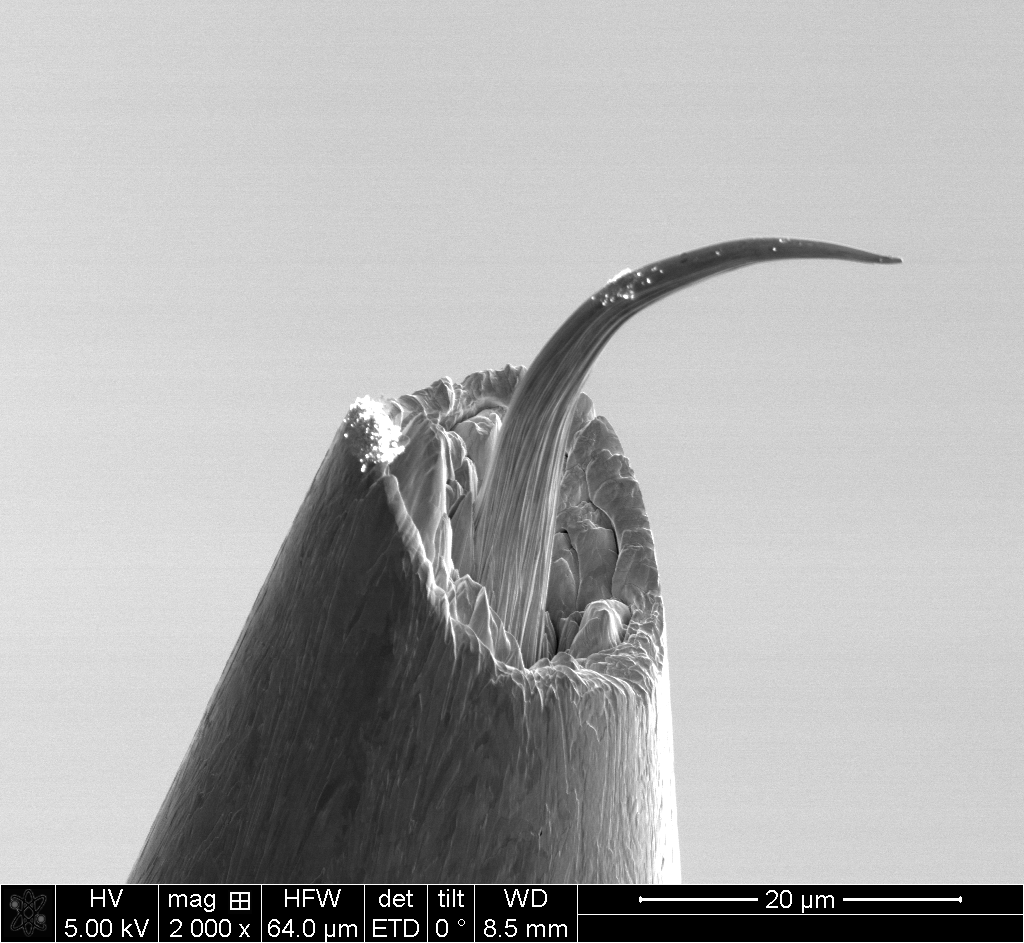
\includegraphics[trim = 0 0 0 0,  clip= true, width = \textwidth]{./pics/M05-13_140826_05.png}}
				\caption{}
				\label{subfig::nanomanipulator_tip_bent}
			\end{subfigure}
			\caption[Detail of nano-manipulator tips]{Detail of tips used as nano-manipulators. The actual tip can be seen projecting out from a bigger supporting structure. (a) Well-formed tip after sharpening. (b) Bend tip, silently attesting to the use of excessive force.}
		\end{figure}

	\subsection{Determination of The Position of \Nds} \label{subsec::position}

		Using the confocal setup detailed in \autoref{ch::pl_setup} we identified \nds containing \sivs suitable for the use in photonic structures. However, to actually move those \nds to a target photonic structure the SEM setup described in the previous section must be used. This implies that after substrates containing suitable \nds are mounted in the SEM setup, the same \nds must be located on the substrate in order for the nano-manipulator to address them correctly.
		To facilitate this and help locate relevant \nds, $\SI{10}{\micro\meter\squared}$ cross markers with a nominal depth of \SI{40}{\nm} were milled into the \ir coating of the \si substrate using the \fib prior to spin-coating the substrate with \nd solution. The markers were arranged in a regular $11 \times 11$ grid covering an area of $\SI{0.5}{\milli\meter} \times \SI{0.5}{\milli\meter}$. \autoref{subfig::cross_markers} illustrates a sample array. Typically three arrays of markers were milled per substrate used.

		\begin{figure}[htp]
			\begin{subfigure}[t]{ 0.49\linewidth}
				\centering
				\testbox{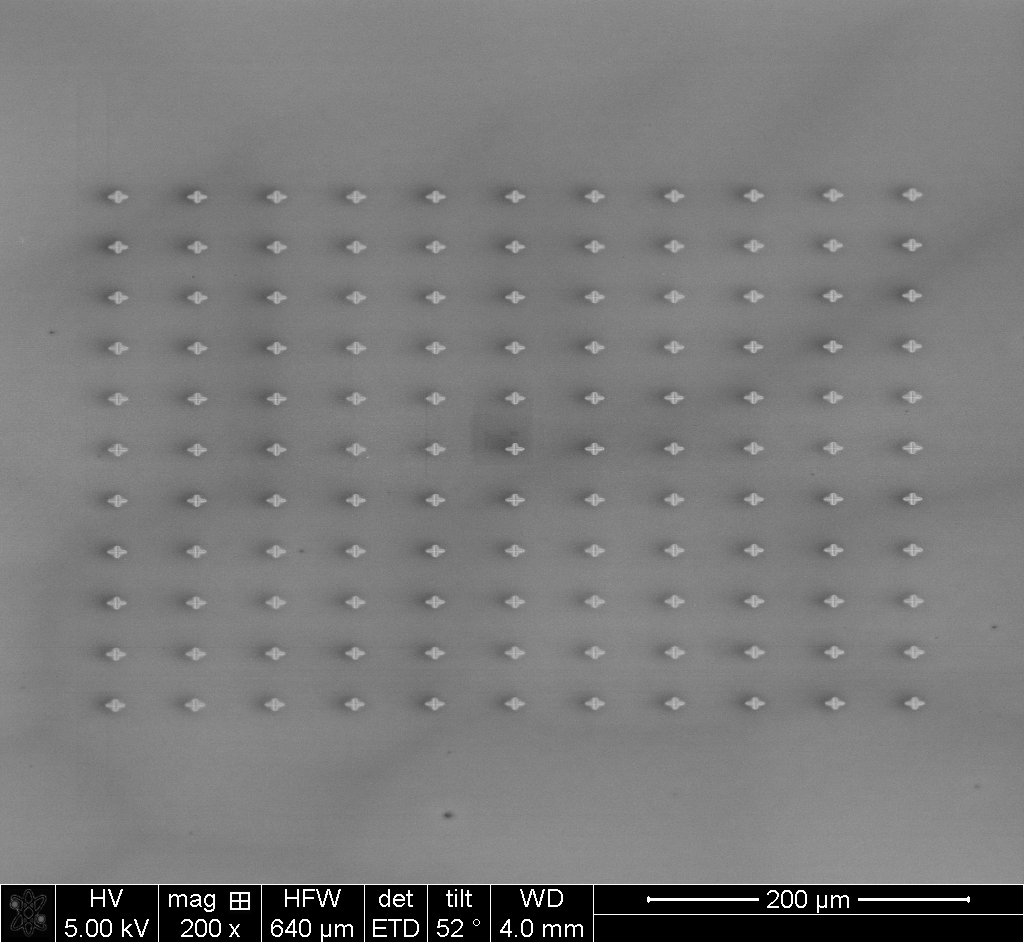
\includegraphics[trim = 0 0 0 0,  clip= true, height = 0.7\textwidth]{./pics/M09-13_mitte_131209_01.png}}
				\caption{}
				\label{subfig::cross_markers}
			\end{subfigure}
			\hfill
			\begin{subfigure}[t]{ 0.49\linewidth}
				\centering
				\testbox{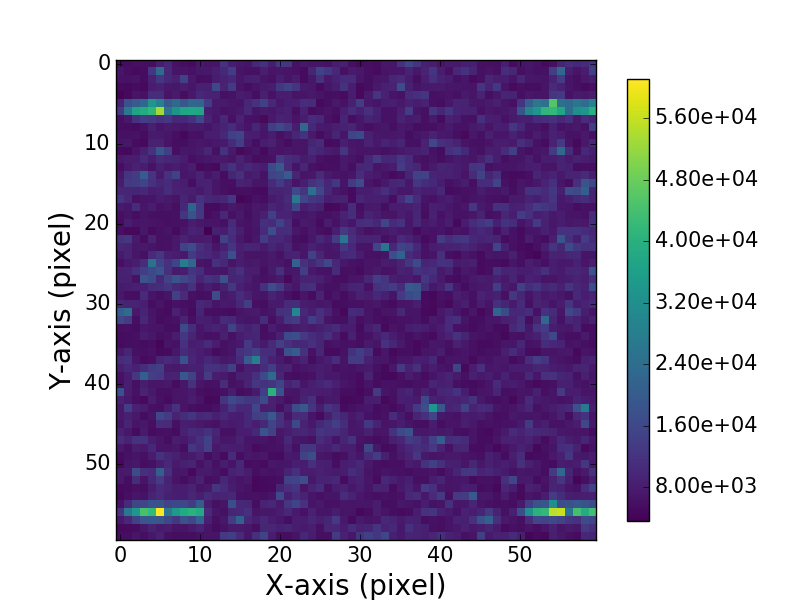
\includegraphics[trim = 0 0 0 0,  clip= true, height = 0.7\textwidth]{./pics/114-02_2APD.png}}
				\caption{}
				\label{subfig::cross_marker_whitelightscan}
			\end{subfigure}
			\caption[Cross markers assisting identification of \nds]{(a) Top-view of a regular array of cross markers. (b) White light scan of an area. Cross markers can be seen in an all four corners.}
		\end{figure}


		To record the position of a \nd \wrt a cross marker, we used two different methods:

		In the first method the confocal setup is used with a white light source illuminates the sample from the side at an acute angle. As a result, the edges of the cross markers become visible in the \fl scan, see \autoref{subfig::cross_marker_whitelightscan}. After turning the white light lamp off, the same area is scanned again to record the fluorescence from the \sivs. An overlay of the two images identifies the position of fluorescent \sivs \wrt the cross markers. The disadvantage of this method is the increased time consumption, as every scan for every subregion of the sample has to be performed twice. As only \fl scans are performed, no information about the size of individual \nds is available. Furthermore, it remains unknown whether \nds are present in isolation or close to each other. Such information is only available in the SEM where the \pp is conducted. It is only at this later stage, that individual \nds can be excluded as unusable for the \pp process. For such \nds the time spend of characterizing its properties was unfortunately wasted.

		To mitigate this problem, a more efficient method consists of scanning the substrate first using a commercial \lsm. The \lsm is a confocal microscope where the focus of a laser can be used to obtain the height of a structure. When scanning an array of cross markers a gray-scale image is obtained, where the gray value corresponds to the height deviation of a structure. As a result, both the crosses with a nominal depth of \SI{40}{\nm} and the \nds themselves are revealed as darker shades of gray. In contrast to the previous method, information on the size and isolation of \nds is accessible. After scanning the substrate with the \lsm, it is inserted into the confocal setup. While observing the surface with a CCD camera, a specific cross marker is chosen as the starting point for a \fl scan. Comparing the \lsm image and a \fl scan, fluorescent dots of the \fl scan can be attributed to \nds in the \lsm scan. \autoref{subfig::cross_laser_scan,subfig::pp_pl_scan} illustrate the process.

		\begin{figure}[htp]
			\begin{subfigure}{ 0.49\linewidth}
				\centering
				\testbox{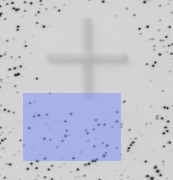
\includegraphics[trim = 0 0 0 0,  clip= true, height = 0.7\textwidth]{./pics/M05-13_structure3_stitch_crop_area.jpg}}
				\caption{}
				\label{subfig::cross_laser_scan}
			\end{subfigure}
			\hfill
			\begin{subfigure}{ 0.49\linewidth}
				\centering
				\testbox{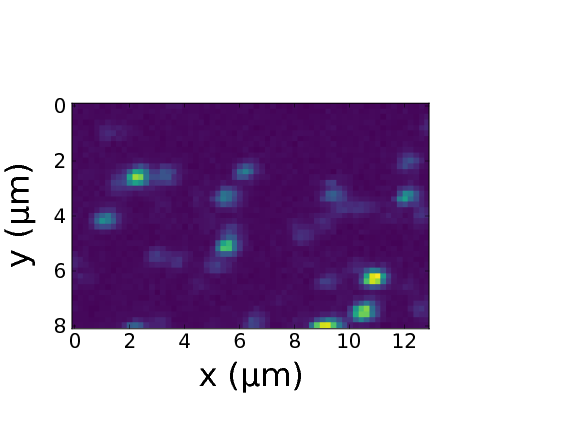
\includegraphics[trim = 0 20 70 50,  clip= true, height = 0.7\textwidth]{./pics/scan_xy-32_2APD_mum_noscale.png}}
				\caption{}
				\label{subfig::pp_pl_scan}
			\end{subfigure}
				\caption[Combining \fl and \lsm to identify \nds]{a) Picture recorded with a commercial high resolution laser scanning microscope. Cross marker is visible as well. b) \Pl scan of a $\SI{8}{\micro\metre} \times  \SI{13}{\micro\metre}$ corresponding to the blue shaded area in b).he area shaded in blue represents the \pl scan in image b).}
		\end{figure}


	\subsection{The \PP Process}

			The \pp process aims to transfer a select \nd between two substrates using the tip mounted inside a \sem. The advantage of using the SEM tip as a nano-manipulator lies in the fact that the progress of the manipulation process can be visualized directly, allowing for a better control of the operation. \autoref{fig::pp_sketch} illustrates the process.

			\begin{figure}[htp]
				\centering
				\testbox{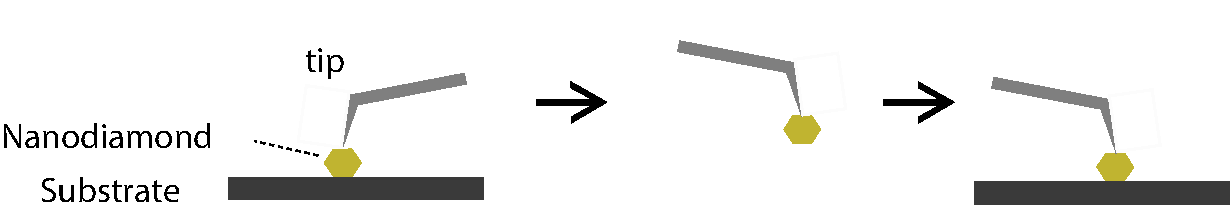
\includegraphics[trim = 0 0 0 0,  clip= true, width = 0.7\textwidth]{./pics/pp_sketch.pdf}}
				\caption{Sketch of the \pp process}
				\label{fig::pp_sketch}
			\end{figure}

	After we identified \nds as well-suited for transfer to the target structure, both the substrate with the \nds and the target structure were mounted inside the SEM.
	The process was performed using a high resolution mode with a low acceleration voltage of the SEM of \SI{1}{\kilo\electronvolt} and a current of \SI{1.7}{\nano\ampere}.
	The tip is approaching the target preselected \nd from above.
	As the SEM objective is mounted above the \np, the proximity the \np tip  to the \nd is not observable.
	To enable the tip of the nano-manipulator to pick up a target \nd a precise approach is necessary. To facilitate this difficult procedure, the approach is divided into two stages: A coarse stage and a fine stage.

	In the coarse stage the distance between tip and target \nd is indirectly estimated from the shadow the tip itself casts onto the substrate and the focus area. As the tip approaches the target, the shadow of the tip starts to coincide with the \nd position. At this point the fine stage of the approach begins in order to cover the remaining distance. To precisely control the final approach the focus of the SEM is used. Note that, as the distance between the tip and the target decreases, the focus must become sharp. Note that if the SEM is focused on the \nd, the tip is out of focus and appears blurry. However, as the distance between the tip and the target decreases, the focus must become sharp. Thus the tip must be moved with utmost care until the focus becomes sharp at which point the tip touches the \nd and pick-up can commence. While the process appears straightforward in concept, it is extremely challenging to operate the involved machinery to the required precision. As can be seen in \autoref{subfig::nanomanipulator_tip_bent} it is easy to overshoot the target and to ruin the tip in the process.
	\\
	When performed correctly, the \nd sticks to the tip due to adhesion when the both get in contact, see \autoref{subfig::pick_antenna_sem_intro}.
	The nano-manipulator is then moved to the target structure and the approach procedure is applied in reverse. \autoref{subfig::transfer_antenna_sem_intro} illustrates the tip of the nano-manipulator carrying a \nd towards its destination structure.
	Depending on the material of the target structure, the \nd either sticks to the structure right away due to higher adhesion forces between the \nd and the structure (as is the case for golden plasmonic antennas).
	Alternatively, a sideways motion of the \np tip must be used in an attempt to strike-off the \nd.
	Either way, with patience it is possible to place a \nd in a target position within a precision of a few nanometers.
	\\

	\begin{figure}[htp]
		\begin{subfigure}[t]{ 0.49\linewidth}
			\centering
			\testbox{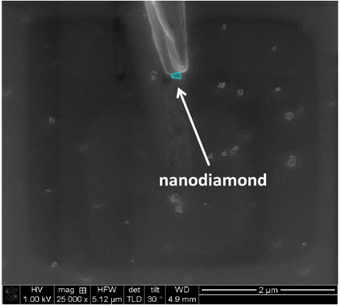
\includegraphics[trim = 0 0 0 0,  clip= true, height = 0.7\textwidth]{./pics/pick_colored.png}}
			\caption{}
			\label{subfig::pick_antenna_sem_intro}
		\end{subfigure}
		\hfill
		\begin{subfigure}[t]{ 0.49\linewidth}
			\centering
			\testbox{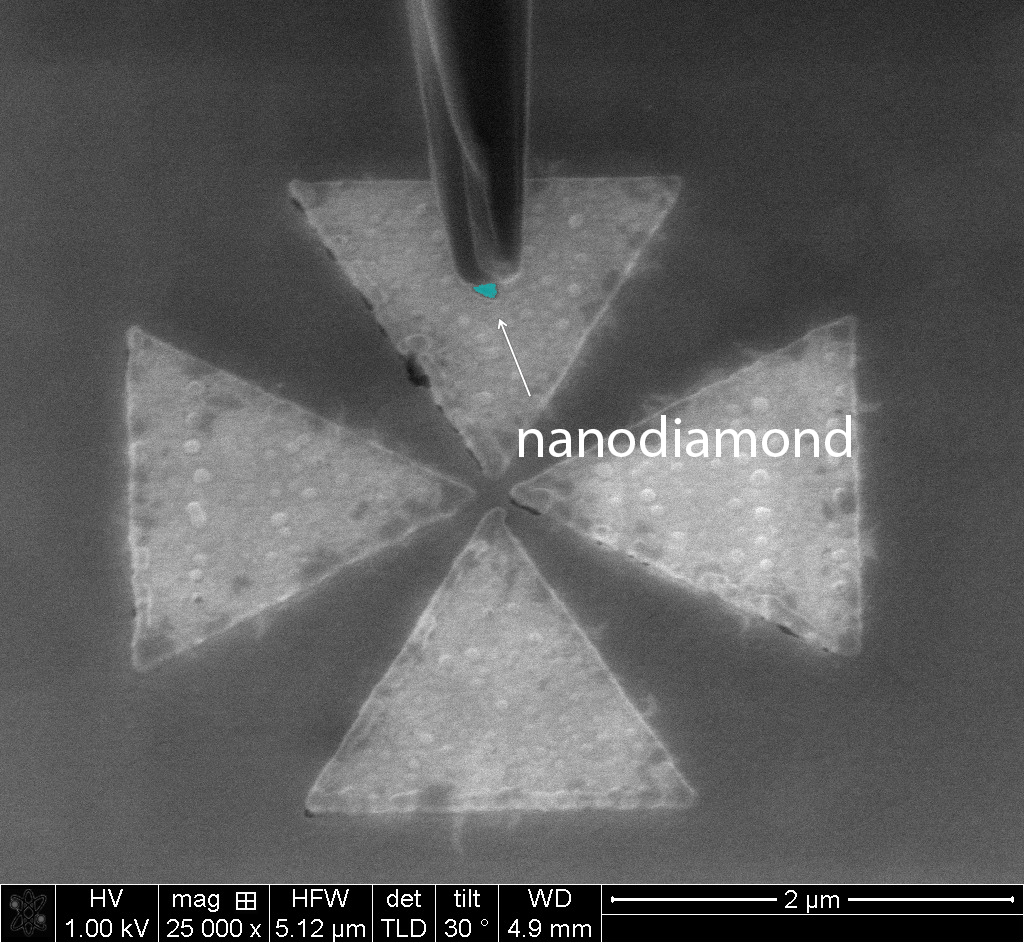
\includegraphics[trim = 0 0 0 0,  clip= true, height = 0.7\textwidth]{./pics/Ir27M_mitte_213_151111_26_colored.png}}
			\caption{}
			\label{subfig::transfer_antenna_sem_intro}
		\end{subfigure}
		\caption[Nano-manipulator carrying a \nd]{a) Tip of the nano-manipulator after successful pick-up of a \nd. b) Tip of the loaded nano-manipulator approaching the target structure about to deliver a \nd.}
	\end{figure}



	% The used SEM has a special high resolution mode.
	% With this mode it is possible, to obtain high resolution images at a low acceleration voltage.
	% The pitfall is that for this mode a small working distance of \SI{5}{mm} is necessary.
	% This working distance is too small for to use the nanomanipulator at the same time.
	% Therefore, first we identified the position of the pre-selected \nd in high resolution mode in the SEM, marked its position in the iamge, switched to normal working mode and
	% - Hochaufloesungsmodus geringer arbeitsabstand von 5mm, higher magn. field
	% - Abloesen von Diamanten (BASD + CVD) von Substrat im Ultraschallbad kann dazu fuehren, dass Substrat mitabgeloest wird) -> in Kalilauge aufloesen LII, S96
	% - warum nicht einfach neue CVD-Diamanten herstellen, wie die, die am Anfang meiner Diss so gut funktioniert haben -> Dichte am Substrat zu hoch zum Aufpicken
